
%??ds caption consistency?, but make captions "better" as per comments

\section{Magnetisation renormalisation methods}
\label{sec:magn-renorm-meth}

We compare renormalisation after every step with the methods used to achieve constant $\abs{\mv}$ in \nmag and \magpar.

We use fixed step BDF2 with step sizes of $\dtn = 0.1$ and a Newton-Raphson tolerance of $\ntol = 10^{-8}$ unless otherwise specified.
We choose BDF2 for these experiments because TR is equivalent to IMR for the undamped ODE LLG problem, and so could be expected to show some geometric integration properties.

\subsection{Renormalisation after a tolerance}
\label{sec:renorm-after-toler}

\newcommand{\mltol}{\epsilon_{\mathrm{ml}}}

\begin{figure}
  \centering
  \includegraphics[width=0.8\textwidth]{{{plots/tolrenorm-geom-properties/0.01-mlengtherrormaxesvstimes}}}
  \caption{
    Error in magnetisation length against time
    for the ODE LLG problem
    with $\dampc = 0.01$.
    The legend indicates the values of $\mltol$, the tolerance on the magnetisation length after which the magnetisation is re-normalised.
  }
  \label{fig:renorm-tol-ml-err}
\end{figure}

\begin{figure}
  \centering
  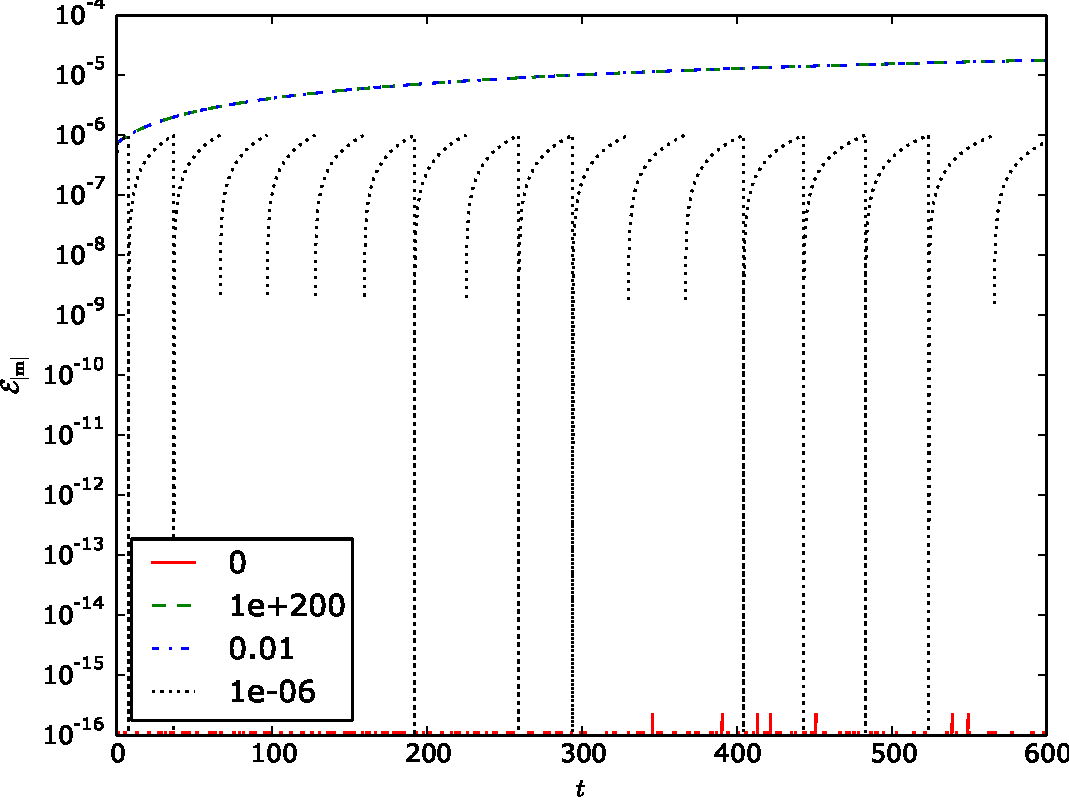
\includegraphics[width=0.8\textwidth]{{{plots//tolrenorm-geom-properties/0-mlengtherrormaxesvstimes}}}
  \caption{
    Error in magnetisation length against time
    for the ODE LLG problem with
    $\dampc = 0$.
    The legend indicates the values of $\mltol$, the tolerance after which the magnetisation is re-normalised.
  }
  \label{fig:renorm-tol-ml-err-undamped}
\end{figure}

In \cref{fig:renorm-tol-ml-err,fig:renorm-tol-ml-err-undamped} we show the error in the magnetisation length over time for various values of $\mltol$ for the damped and undamped problems respectively.
Note that $\mltol = 10^{200}$ results in no renormalisation being carried out ever, while $\mltol = 0$ results in re-normalisation after every time step.
In both the damped and undamped cases, the use of the intermediate tolerance value, $\mltol = 10^{-6}$, results in oscillations of the magnetisation length.
In the undamped case with $\mltol = 10^{-2}$ the error in the magnetisation length never reaches the tolerance, and so the behaviour is identical to no renormalisation.
In the damped case $\mltol = 10^{-2}$ is reached and the behaviour is similar to that of $\mltol = 10^{-6}$, except that the oscillations begin at a later time.

??ds why are there oscillations? Renorm induces so much error that it swings right back up? Possibly we should be doing something to the history values as well?

\begin{figure}
  \centering
  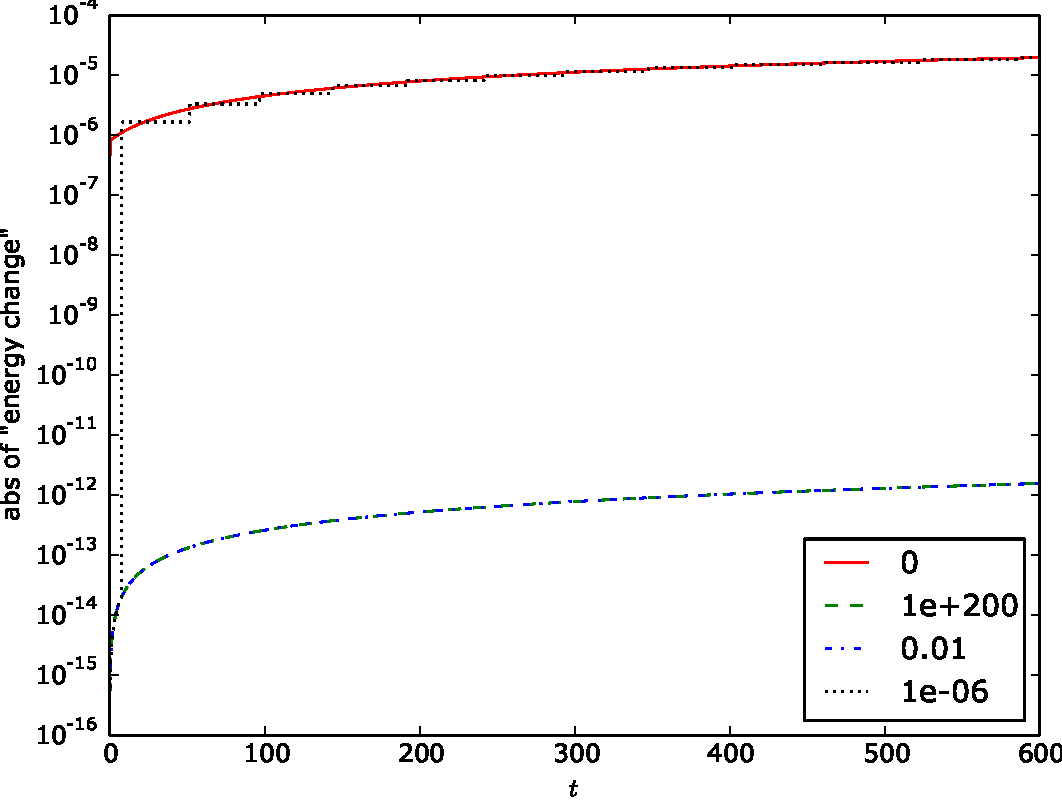
\includegraphics[width=0.8\textwidth]{plots/tolrenorm-geom-properties/0-absofenergychangevstimes.pdf}
  \caption{
    Error in energy against time
    for the ODE LLG problem
    with $\dampc = 0$.
    The legend indicates the values of $\mltol$, the tolerance after which the magnetisation is re-normalised.
  }
  \label{fig:renorm-tol-energy-err}
\end{figure}

In \cref{fig:renorm-tol-energy-err} the errors in the energy for the undamped case are shown.
As noted previously, $\mltol= 10^{-2}$ behaves as the non-renormalised case for this example.
When $\mltol = 10^{-6}$ we see an error similar to that for the always renormalised case, except with additional oscillations in the energy corresponding to times where a renormalisation is carried out.


\begin{figure}
  \centering
  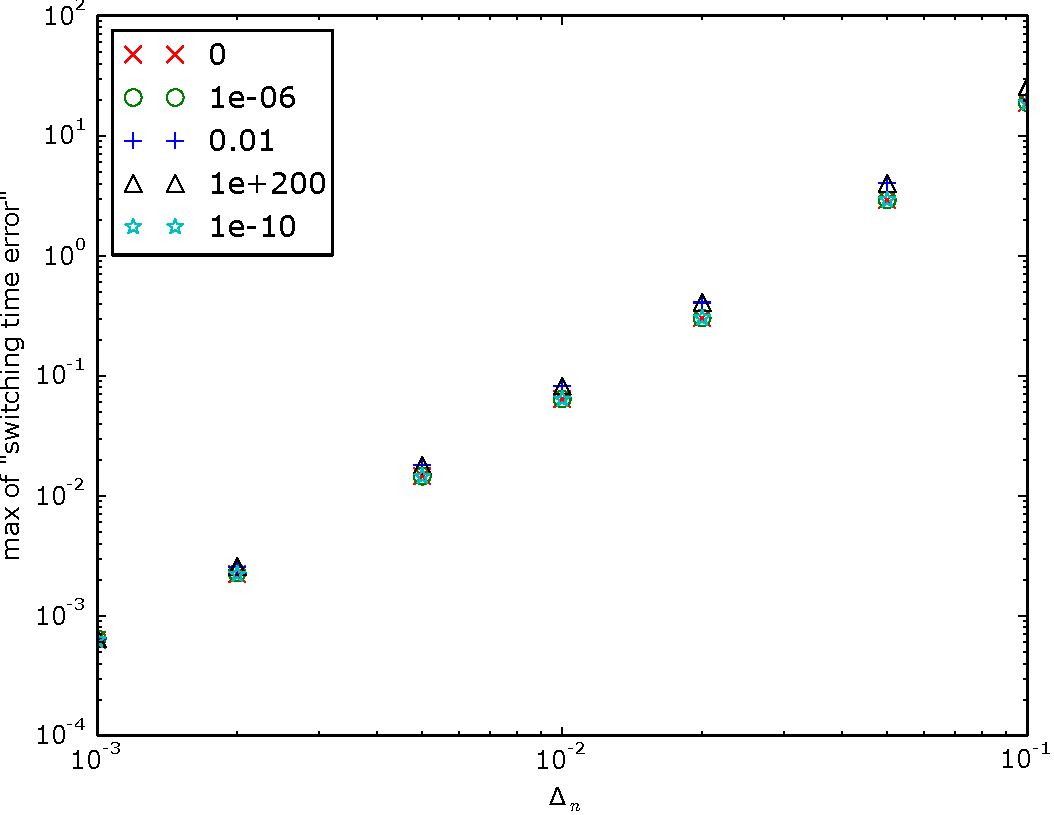
\includegraphics[width=0.8\textwidth]{plots/tolrenorm_llg_ode_convergence/maxofswitchingtimeerrorvsmeanofdts}
  \caption{
    Convergence of the maximum (over all steps) of the error in the switching time
    against step size
    for the ODE LLG problem with
    $\dampc = 0.01$.
    The legend indicates the tolerance after which the magnetisation is re-normalised.
    ??ds not actually a mean...
  }
  \label{fig:tol-renorm-convergence}
\end{figure}

Finally in \cref{fig:tol-renorm-convergence} we show the convergence of the method (in terms of the error in the switching time) for the damped case as the step size is reduced.
It can be seen that the $\mltol=10^{-2}$ or no renormalisation gives slightly worse errors for large step sizes than the tighter magnetisation length tolerances.

??ds add more intermediate tolerances?


\subsection{The self-correcting LLG}
\label{sec:self-correcting-llg-results}

The self correcting parameter $\scc = 0, 0.1, 1, 10, 100, 1000$, larger values were not used because the Newton-Raphson method began to fail to converge within ten steps.

For comparison we also show plots using IMR, with Newton tolerance $\ntol=10^{-12}$ (recall that a sharp linearisation tolerance is required for IMR to attain good geometric integration properties).


\begin{figure}
  \centering
  \includegraphics[width=0.8\textwidth]{{{plots/self_correcting_ode/0.01-mlengtherrormaxesvstimes}}}
  \caption{
    Error in magnetisation length against time
    for the ODE self-correcting LLG problem
    with $\dampc = 0.01$.
    The legend indicates the values of $\scc$.
  }
  \label{fig:sc-ml-err}
\end{figure}


\begin{figure}
  \centering
  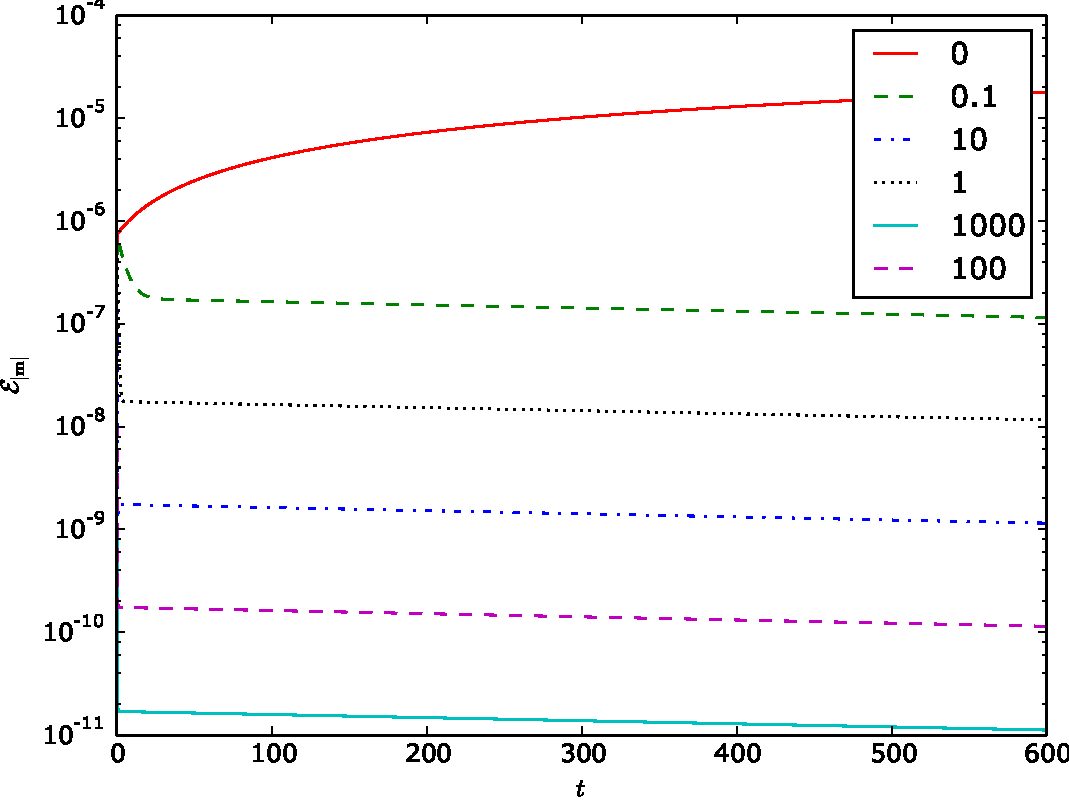
\includegraphics[width=0.8\textwidth]{plots//self_correcting_ode/0-mlengtherrormaxesvstimes.pdf}
  \caption{
    Error in magnetisation length against time for the ODE self-correcting LLG problem with
    $\dampc = 0$.
    The legend indicates the values of $\scc$.
  }
  \label{fig:sc-ml-err-undamped}
\end{figure}

\begin{figure}
  \centering
  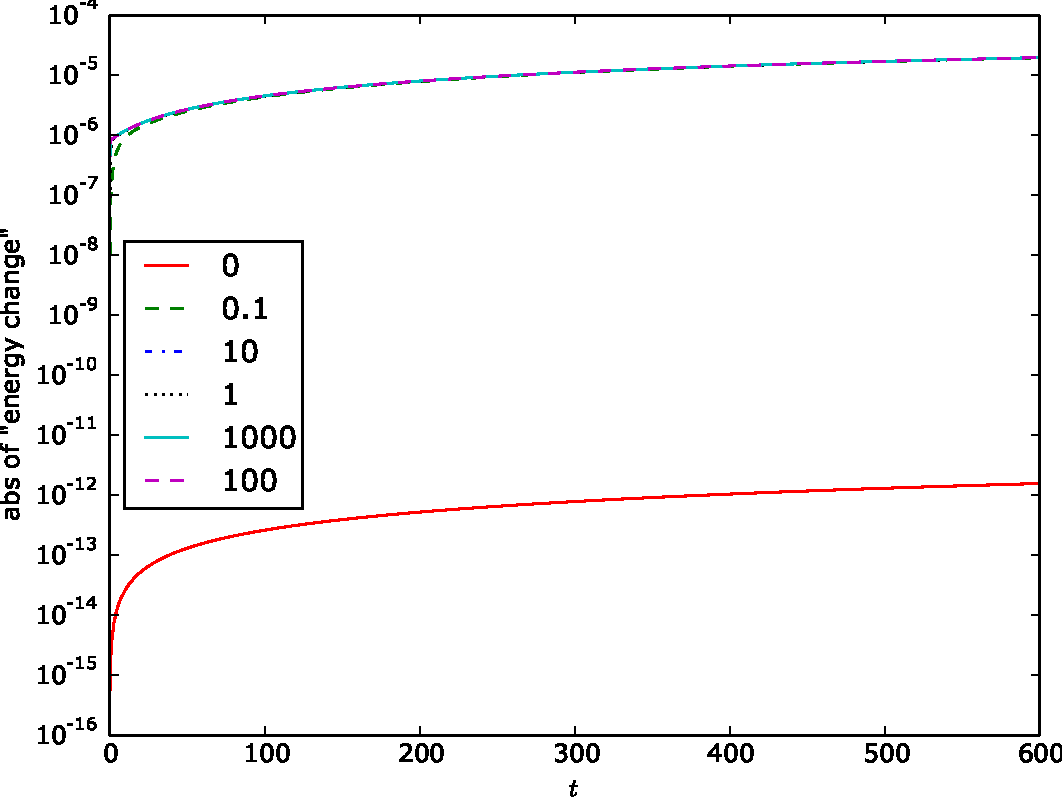
\includegraphics[width=0.8\textwidth]{plots/self_correcting_ode/0-absofenergychangevstimes.pdf}
  \caption{
    Error in energy against time
    for the ODE self-correcting LLG problem
    with $\dampc = 0$.
    The legend indicates the values of $\scc$.
  }
  \label{fig:sc-energy-err}
\end{figure}


Also show IMR iters?
\begin{figure}
  \centering
  % \includegraphics[width=0.8\textwidth]{plots/self_correcting_ode/??ds}
  \caption{
    Number of Newton-Raphson iterations to converge to $\ntol = 10^{-8}$ against the parameter $\scc$
    for the ODE self-correcting LLG problem
    with $\dampc = 0.01$.
    Also shown is the number of iterations to converge to $\ntol = 10^{-12}$ with IMR. ??ds
  }
  \label{fig:sc-newt-iters}
\end{figure}

Show error or switching time error?
\begin{figure}
  \centering
  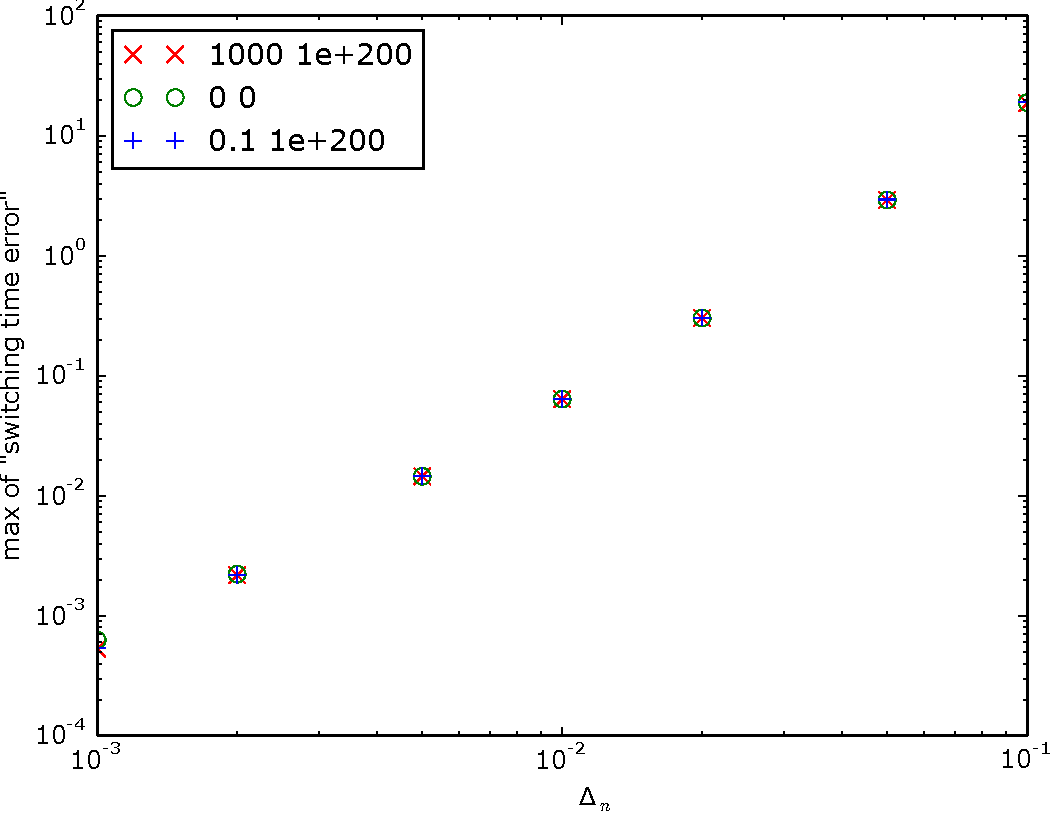
\includegraphics[width=0.8\textwidth]{plots/self_correcting_llg_ode_convergence/maxofswitchingtimeerrorvsmeanofdts}
  \caption{
    Convergence of the maximum (over all steps) of the error in the switching time
    against step size
    for the ODE self-correcting LLG problem with
    $\dampc = 0.01$.
    The legend indicates, respectively, the values of $\scc$ and the tolerance after which the magnetisation is re-normalised.
  }
  \label{fig:sc-convergence}
\end{figure}

\subsection{Conclusions}

Renormalisation after a tolerance allows larger errors in $\abs{\mv}$ than renorm after each step (by definition).
It also introduces spurious oscillations in $\abs{\mv}$.
Effect on convergence ??ds
In terms of computational cost: checking whether renormalisation is needed has roughly the same cost as actually renormalising.
Hence there is no reason to prefer renormalisation after a tolerance.


Self correcting LLG is always worse in controlling GI errors than renorm after each step: energy errors the same, m errors much larger.
It also takes additional newton step(s) (typically one more step is needed, increasing the computational time for the simulation by a factor of $\sim 3/2$).
Effect on convergence? ??ds
As such there appears to be no reason to use the self-correcting LLG over renormalisation after each step.

%%% Local Variables:
%%% mode: latex
%%% TeX-master: "main"
%%% End:
